% -*- mode: noweb; ess-noweb-default-code-mode: lisp-mode; -*-% ===> this file was generated automatically by noweave --- better not edit it
\documentclass{tufte-handout}

\usepackage{fontspec}
% https://tex.stackexchange.com/a/43628/45537
\setmainfont[Mapping=tex-text,Numbers=OldStyle]{Palatino}
\setsansfont[Mapping=tex-text,Numbers=OldStyle,Scale=MatchLowercase]{Gill Sans}
\setmonofont[Mapping=tex-text,Scale=MatchLowercase]{Iosevka}

% HACK: https://tex.stackexchange.com/a/200725/45537
\usepackage{ifxetex}
\ifxetex
  \newcommand{\textls}[2][5]{%
    \begingroup\addfontfeatures{LetterSpace=#1}#2\endgroup
  }
  \renewcommand{\allcapsspacing}[1]{\textls[15]{#1}}
  \renewcommand{\smallcapsspacing}[1]{\textls[10]{#1}}
  \renewcommand{\allcaps}[1]{\textls[15]{\MakeTextUppercase{#1}}}
  \renewcommand{\smallcaps}[1]{\smallcapsspacing{\scshape\MakeTextLowercase{#1}}}
  \renewcommand{\textsc}[1]{\smallcapsspacing{\textsmallcaps{#1}}}
\fi

\usepackage{noweb}
\noweboptions{smallcode,longxref,webnumbering,longchunks,english}

\usepackage{color}
% https://commons.wikimedia.org/wiki/File:Erlang_logo.svg
\definecolor{ErlangRed}{HTML}{A90533}

\usepackage{amsmath}
\usepackage{amssymb}

\usepackage{mathtools}
\mathtoolsset{centercolon}
\DeclarePairedDelimiter{\floor}{\lfloor}{\rfloor}

\usepackage{dirtytalk}

\usepackage[english]{fancyref}

\usepackage[outputdir=src]{minted}
\newmintinline[lsp]{lisp}{}
\newmintinline[cee]{c}{}

\usepackage{hyperref}
\newcommand{\srclink}[1]{%
  \href{https://github.com/yurrriq/land-of-lisp/blob/master/#1}{%
    \mintinline{text}{#1}%
  }%
}

\author{Eric Bailey}

\hypersetup{
  pdffitwindow=true,
  pdfstartview={FitH},
  pdftitle={Pudding Eater},
  pdfauthor={Eric Bailey <eric@ericb.me>},
  pdfsubject={Land of Lisp: Chapter 4},
  pdfkeywords={Lisp, silly, literate programming, noweb},
  colorlinks=true,
  linkcolor=ErlangRed,
  urlcolor=ErlangRed
}

\title{%
  Pudding Eater
  \thanks{\cite{barski2010land-ch4}}
}

\date{%
  October 10, 2017
  \thanks{Last updated \today}
}

\begin{document}
\maketitle
\nwfilename{src/pudding.nw}\nwbegindocs{1}\nwdocspar

% \begin{abstract}
%   Who ate my pudding?
% \end{abstract}

% \tableofcontents
% \newpage


\section{Defining the Arch-Enemy Variable}

Since at first we don't know who the pudding eater (a.k.a. our {\Tt{}\nwlinkedidentq{*arch-enemy*}{NWlm77s-1p0Y9w-1}\nwendquote})
is, set the initial value to \lsp{nil}.

\marginnote[1.5\baselineskip]{%
  \say{Global variable names should start and end with asterisks (also known in
    this context as earmuffs)} \citep{google-style-guide}.
}

\nwenddocs{}\nwbegincode{2}\sublabel{NWlm77s-1p0Y9w-1}\nwmargintag{{\nwtagstyle{}\subpageref{NWlm77s-1p0Y9w-1}}}\moddef{*~{\nwtagstyle{}\subpageref{NWlm77s-1p0Y9w-1}}}\endmoddef\nwstartdeflinemarkup\nwprevnextdefs{\relax}{NWlm77s-1p0Y9w-2}\nwenddeflinemarkup
(defvar \nwlinkedidentc{*arch-enemy*}{NWlm77s-1p0Y9w-1} nil)\nwindexdefn{\nwixident{*arch-enemy*}}{*arch-enemy*}{NWlm77s-1p0Y9w-1}


\nwalsodefined{\\{NWlm77s-1p0Y9w-2}}\nwnotused{*}\nwidentdefs{\\{{\nwixident{*arch-enemy*}}{*arch-enemy*}}}\nwendcode{}\nwbegindocs{3}\nwdocspar


\section{Defining the Pudding-Eater Function}

This chapter introduces \lsp{cond}, an extremely versatile function that's
\say{been around sine the Lisp Stone Age.} The basic form is as follows.

\begin{minted}{lisp}
(cond (test-form form*)
      ...)
\end{minted}

\begin{marginfigure}
  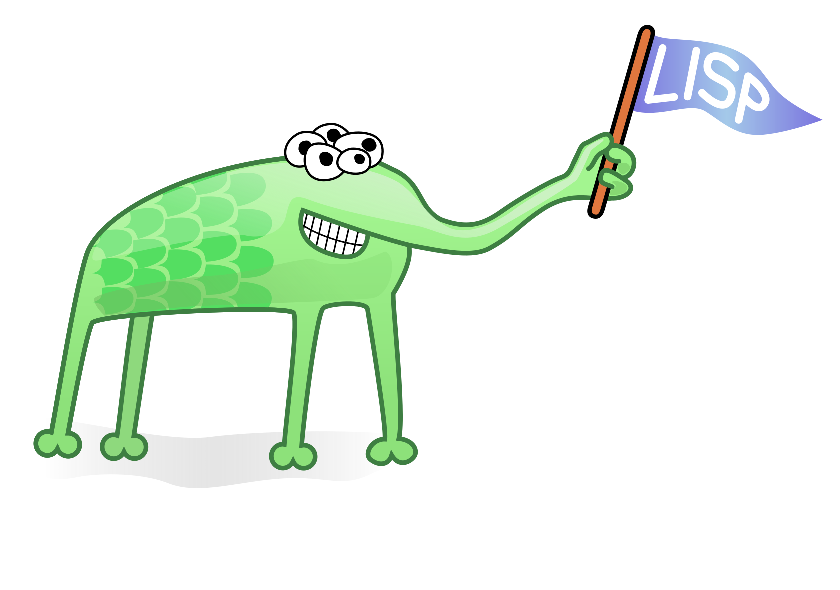
\includegraphics[width=\textwidth]{lisplogo_alien.eps}
  \caption{Henry, the Lisp Alien}
  \label{fig:lisp-alien}
\end{marginfigure}

Since \lsp{test-form}s are evaluated for truthiness, we can branch on which
\lsp{person} ate our pudding.

\begin{marginfigure}
\nwenddocs{}\nwbegincode{4}\sublabel{NWlm77s-e7MAZ-1}\nwmargintag{{\nwtagstyle{}\subpageref{NWlm77s-e7MAZ-1}}}\moddef{it was Henry~{\nwtagstyle{}\subpageref{NWlm77s-e7MAZ-1}}}\endmoddef\nwstartdeflinemarkup\nwusesondefline{\\{NWlm77s-2TVrZS-1}}\nwenddeflinemarkup
(eq person 'henry)
\nwused{\\{NWlm77s-2TVrZS-1}}\nwendcode{}\nwbegindocs{5}\nwdocspar

\nwenddocs{}\nwbegincode{6}\sublabel{NWlm77s-155yI6-1}\nwmargintag{{\nwtagstyle{}\subpageref{NWlm77s-155yI6-1}}}\moddef{blame Henry~{\nwtagstyle{}\subpageref{NWlm77s-155yI6-1}}}\endmoddef\nwstartdeflinemarkup\nwusesondefline{\\{NWlm77s-2TVrZS-1}\\{NWlm77s-1p0Y9w-2}}\nwenddeflinemarkup
(setf \nwlinkedidentc{*arch-enemy*}{NWlm77s-1p0Y9w-1} 'stupid-lisp-alien)
'(curse you lisp alien - you ate my pudding)
\nwused{\\{NWlm77s-2TVrZS-1}\\{NWlm77s-1p0Y9w-2}}\nwidentuses{\\{{\nwixident{*arch-enemy*}}{*arch-enemy*}}}\nwindexuse{\nwixident{*arch-enemy*}}{*arch-enemy*}{NWlm77s-155yI6-1}\nwendcode{}\nwbegindocs{7}\nwdocspar
\end{marginfigure}

If {\Tt{}\LA{}it was Henry~{\nwtagstyle{}\subpageref{NWlm77s-e7MAZ-1}}\RA{}\nwendquote}, the Lisp alien, {\Tt{}\LA{}blame Henry~{\nwtagstyle{}\subpageref{NWlm77s-155yI6-1}}\RA{}\nwendquote};

\begin{marginfigure}
\nwenddocs{}\nwbegincode{8}\sublabel{NWlm77s-23wlyr-1}\nwmargintag{{\nwtagstyle{}\subpageref{NWlm77s-23wlyr-1}}}\moddef{it was Johnny~{\nwtagstyle{}\subpageref{NWlm77s-23wlyr-1}}}\endmoddef\nwstartdeflinemarkup\nwusesondefline{\\{NWlm77s-2TVrZS-1}}\nwenddeflinemarkup
(eq person 'johnny)
\nwused{\\{NWlm77s-2TVrZS-1}}\nwendcode{}\nwbegindocs{9}\nwdocspar

\nwenddocs{}\nwbegincode{10}\sublabel{NWlm77s-3I6gnZ-1}\nwmargintag{{\nwtagstyle{}\subpageref{NWlm77s-3I6gnZ-1}}}\moddef{blame Johnny~{\nwtagstyle{}\subpageref{NWlm77s-3I6gnZ-1}}}\endmoddef\nwstartdeflinemarkup\nwusesondefline{\\{NWlm77s-2TVrZS-1}\\{NWlm77s-1p0Y9w-2}}\nwenddeflinemarkup
(setf \nwlinkedidentc{*arch-enemy*}{NWlm77s-1p0Y9w-1} 'useless-old-johnny)
'(i hope you chocked on my pudding johnny)
\nwused{\\{NWlm77s-2TVrZS-1}\\{NWlm77s-1p0Y9w-2}}\nwidentuses{\\{{\nwixident{*arch-enemy*}}{*arch-enemy*}}}\nwindexuse{\nwixident{*arch-enemy*}}{*arch-enemy*}{NWlm77s-3I6gnZ-1}\nwendcode{}\nwbegindocs{11}\nwdocspar
\end{marginfigure}

If {\Tt{}\LA{}it was Johnny~{\nwtagstyle{}\subpageref{NWlm77s-23wlyr-1}}\RA{}\nwendquote}, {\Tt{}\LA{}blame Johnny~{\nwtagstyle{}\subpageref{NWlm77s-3I6gnZ-1}}\RA{}\nwendquote}.

\begin{marginfigure}
\nwenddocs{}\nwbegincode{12}\sublabel{NWlm77s-I8i5u-1}\nwmargintag{{\nwtagstyle{}\subpageref{NWlm77s-I8i5u-1}}}\moddef{ask them why~{\nwtagstyle{}\subpageref{NWlm77s-I8i5u-1}}}\endmoddef\nwstartdeflinemarkup\nwusesondefline{\\{NWlm77s-2TVrZS-1}\\{NWlm77s-1p0Y9w-2}}\nwenddeflinemarkup
'(why you eat my pudding stranger ?)
\nwused{\\{NWlm77s-2TVrZS-1}\\{NWlm77s-1p0Y9w-2}}\nwendcode{}\nwbegindocs{13}\nwdocspar
\end{marginfigure}

If it was someone else, {\Tt{}\LA{}ask them why~{\nwtagstyle{}\subpageref{NWlm77s-I8i5u-1}}\RA{}\nwendquote}.

The \lsp{cond} version of {\Tt{}\nwlinkedidentq{pudding-eater}{NWlm77s-1p0Y9w-2}\nwendquote} then, would look like this:

\nwenddocs{}\nwbegincode{14}\sublabel{NWlm77s-2TVrZS-1}\nwmargintag{{\nwtagstyle{}\subpageref{NWlm77s-2TVrZS-1}}}\moddef{\code{}cond\edoc{}-flavoured \code{}pudding-eater\edoc{}~{\nwtagstyle{}\subpageref{NWlm77s-2TVrZS-1}}}\endmoddef\nwstartdeflinemarkup\nwenddeflinemarkup
(λ (person)
  (cond (\LA{}it was Johnny~{\nwtagstyle{}\subpageref{NWlm77s-23wlyr-1}}\RA{} \LA{}blame Johnny~{\nwtagstyle{}\subpageref{NWlm77s-3I6gnZ-1}}\RA{})
        (\LA{}it was Henry~{\nwtagstyle{}\subpageref{NWlm77s-e7MAZ-1}}\RA{}  \LA{}blame Henry~{\nwtagstyle{}\subpageref{NWlm77s-155yI6-1}}\RA{})
        (t                \LA{}ask them why~{\nwtagstyle{}\subpageref{NWlm77s-I8i5u-1}}\RA{})))
\nwnotused{[[cond]]-flavoured [[pudding-eater]]}\nwendcode{}\nwbegindocs{15}\nwdocspar

More succinctly, with \lsp{case}, we can define the {\Tt{}\nwlinkedidentq{pudding-eater}{NWlm77s-1p0Y9w-2}\nwendquote} function.

\nwenddocs{}\nwbegincode{16}\sublabel{NWlm77s-1p0Y9w-2}\nwmargintag{{\nwtagstyle{}\subpageref{NWlm77s-1p0Y9w-2}}}\moddef{*~{\nwtagstyle{}\subpageref{NWlm77s-1p0Y9w-1}}}\plusendmoddef\nwstartdeflinemarkup\nwprevnextdefs{NWlm77s-1p0Y9w-1}{\relax}\nwenddeflinemarkup
(defun \nwlinkedidentc{pudding-eater}{NWlm77s-1p0Y9w-2} (person)\nwindexdefn{\nwixident{pudding-eater}}{pudding-eater}{NWlm77s-1p0Y9w-2}
  (case person
        ((henry)   \LA{}blame Henry~{\nwtagstyle{}\subpageref{NWlm77s-155yI6-1}}\RA{})
        ((johnny)  \LA{}blame Johnny~{\nwtagstyle{}\subpageref{NWlm77s-3I6gnZ-1}}\RA{})
        (otherwise \LA{}ask them why~{\nwtagstyle{}\subpageref{NWlm77s-I8i5u-1}}\RA{})))
\nwidentdefs{\\{{\nwixident{pudding-eater}}{pudding-eater}}}\nwendcode{}\nwbegindocs{17}\nwdocspar


\section{Full Listing}

\inputminted{lisp}{src/pudding.lisp}


\section{Example Session}

After loading \srclink{src/pudding.lisp},
you might have {\Tt{}\LA{}a session~{\nwtagstyle{}\subpageref{NWlm77s-2aJKj5-1}}\RA{}\nwendquote} like this:

\begin{marginfigure}
\begin{minted}{shell-session}
$ rlwrap sbcl --load src/pudding.lisp
\end{minted}
\end{marginfigure}

\nwenddocs{}\nwbegincode{18}\sublabel{NWlm77s-2aJKj5-1}\nwmargintag{{\nwtagstyle{}\subpageref{NWlm77s-2aJKj5-1}}}\moddef{a session~{\nwtagstyle{}\subpageref{NWlm77s-2aJKj5-1}}}\endmoddef\nwstartdeflinemarkup\nwenddeflinemarkup
> (\nwlinkedidentc{pudding-eater}{NWlm77s-1p0Y9w-2} 'johnny)
(I HOPE YOU CHOKED ON MY PUDDING JOHNNY)
> \nwlinkedidentc{*arch-enemy*}{NWlm77s-1p0Y9w-1}
USELESS-OLD-JOHNNY
> (\nwlinkedidentc{pudding-eater}{NWlm77s-1p0Y9w-2} 'george-clooney)
(WHY YOU EAT MY PUDDING STRANGER ?)
\nwnotused{a session}\nwidentuses{\\{{\nwixident{*arch-enemy*}}{*arch-enemy*}}\\{{\nwixident{pudding-eater}}{pudding-eater}}}\nwindexuse{\nwixident{*arch-enemy*}}{*arch-enemy*}{NWlm77s-2aJKj5-1}\nwindexuse{\nwixident{pudding-eater}}{pudding-eater}{NWlm77s-2aJKj5-1}\nwendcode{}

\nwixlogsorted{c}{{*}{NWlm77s-1p0Y9w-1}{\nwixd{NWlm77s-1p0Y9w-1}\nwixd{NWlm77s-1p0Y9w-2}}}%
\nwixlogsorted{c}{{\code{}cond\edoc{}-flavoured \code{}pudding-eater\edoc{}}{NWlm77s-2TVrZS-1}{\nwixd{NWlm77s-2TVrZS-1}}}%
\nwixlogsorted{c}{{a session}{NWlm77s-2aJKj5-1}{\nwixd{NWlm77s-2aJKj5-1}}}%
\nwixlogsorted{c}{{ask them why}{NWlm77s-I8i5u-1}{\nwixd{NWlm77s-I8i5u-1}\nwixu{NWlm77s-2TVrZS-1}\nwixu{NWlm77s-1p0Y9w-2}}}%
\nwixlogsorted{c}{{blame Henry}{NWlm77s-155yI6-1}{\nwixd{NWlm77s-155yI6-1}\nwixu{NWlm77s-2TVrZS-1}\nwixu{NWlm77s-1p0Y9w-2}}}%
\nwixlogsorted{c}{{blame Johnny}{NWlm77s-3I6gnZ-1}{\nwixd{NWlm77s-3I6gnZ-1}\nwixu{NWlm77s-2TVrZS-1}\nwixu{NWlm77s-1p0Y9w-2}}}%
\nwixlogsorted{c}{{it was Henry}{NWlm77s-e7MAZ-1}{\nwixd{NWlm77s-e7MAZ-1}\nwixu{NWlm77s-2TVrZS-1}}}%
\nwixlogsorted{c}{{it was Johnny}{NWlm77s-23wlyr-1}{\nwixd{NWlm77s-23wlyr-1}\nwixu{NWlm77s-2TVrZS-1}}}%
\nwixlogsorted{i}{{\nwixident{*arch-enemy*}}{*arch-enemy*}}%
\nwixlogsorted{i}{{\nwixident{pudding-eater}}{pudding-eater}}%
\nwbegindocs{19}\nwdocspar


% \section{Index}
% \nowebindex
% \newpage

% \section{Chunks}
% \nowebchunks

\bibliography{pudding}
\bibliographystyle{plainnat}

\end{document}
\nwenddocs{}
